\title{Chum Populations}

\documentclass[12pt,  one column]{article}
\usepackage{graphicx}
\usepackage{float}

\begin{document}

\section*{Abstract}
To do

\section*{Introduction}

\begin{itemize}

\item PS chum pop gen
\begin{itemize}
\item Population structure
\item life history variation
\item ESA listing - summer chum ESU
\item Effective population size
\end{itemize}

\item Genome scan
\begin{itemize}
\item paired population design
\item map-assisted
\item draw on synteny / orthology
\end{itemize}

\item Genotyping duplicates
\begin{itemize}
\item Legacy of the salmonid WGD
\item uncharacterized regions of the genome
\item first approach in salmon using next-gen seq data.  Method applicable to other species with WGD? 

\end{itemize}

\item Map
\begin{itemize}
\item consensus map w/centromeres
\item synteny
\item annotation
\end{itemize}

\end{itemize}


\section*{Methods}

\subsection*{Population Genetics}
Sequence analysis and genotyping

Genotyping duplicate loci using the dominance coding suggested by Patterson (2006). 
Individual-based analyses
\begin{itemize}
    \item PCAs - How do these two methods compare? - maybe measure info loss?
    \item Formal tests for population structure - tracey-widom stats

\end{itemize}

Population-based analyses
\begin{itemize}
	\item MAF, Heterozygosity
    \item phylogenetic tree
	\item Fst across the genome
    \item Effective population size - 
    
    	Effective population size was estimated for each population using the LD method implemented in the LDNe software package (Waples and Do).  The LD methods estimates average  correlation of alleles at pairs of loci (r2). The mean pairwise r2 value across unlinked loci provides an estimate of contemporary effective population size (WAPLES). The linkage map was used to ensure that only pairs of loci not co-located on a chromosome were used to calculate mean r2. 
    \item Bayescan outlier tests
\end{itemize}

\subsection*{Linkage map}

Sequence analysis and genotyping

Identification of paralogs follows Waples (2015)

Map construction follows McKinney (2015), based off Waples (2015)

Synteny - relation to genetic resources
\begin{itemize}
	\item Chinook salmon
    \item Atlantic salmon
\end{itemize}

\section*{Results}

\subsection*{Population Genetics}

Summarize population relationships
Figure of individual-based 4 PCAs

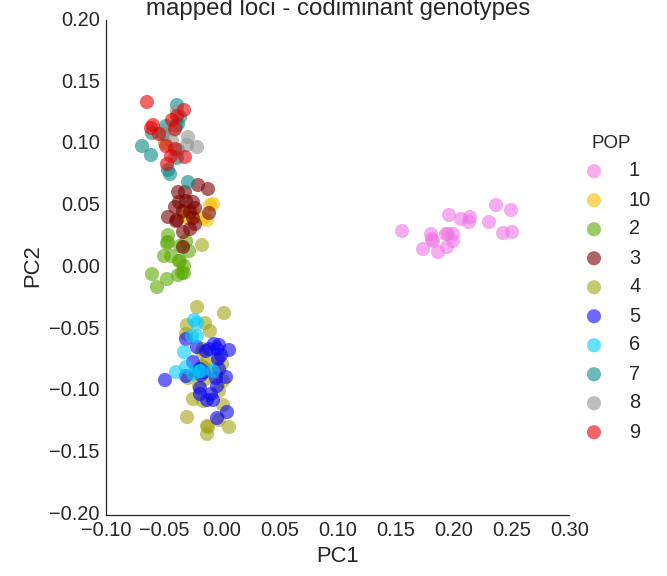
\includegraphics[scale=.3]{figures/PCA_codom.png}
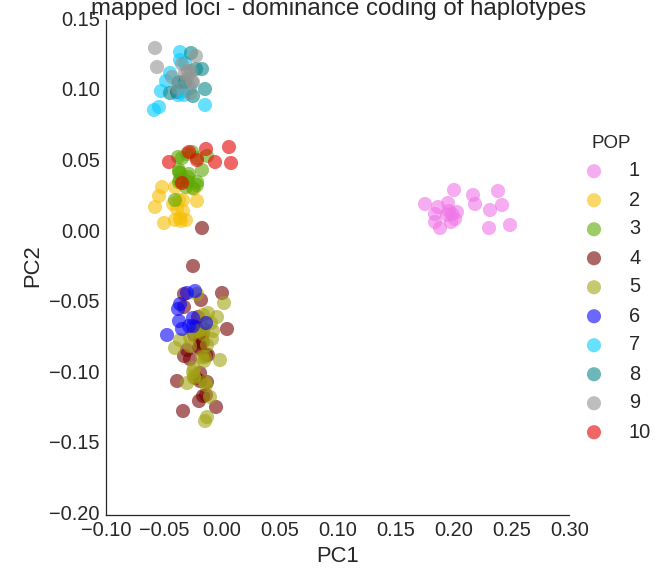
\includegraphics[scale=.3]{figures/PCA_dom.png}

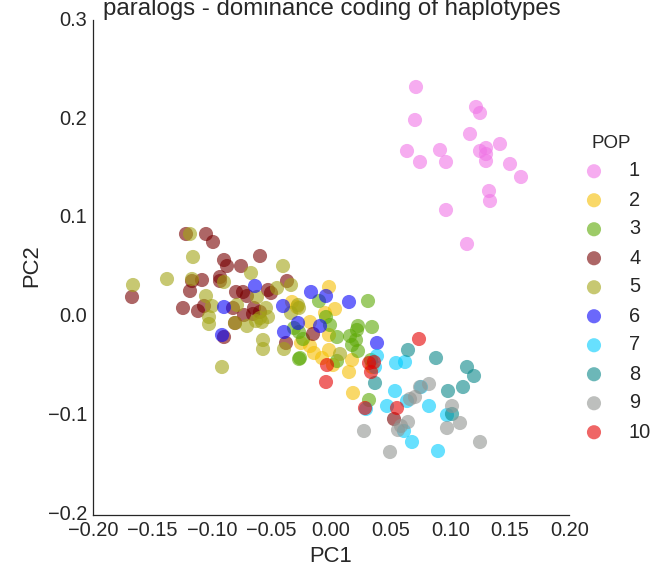
\includegraphics[scale=.3]{figures/PCA_dom_paralogs.png}
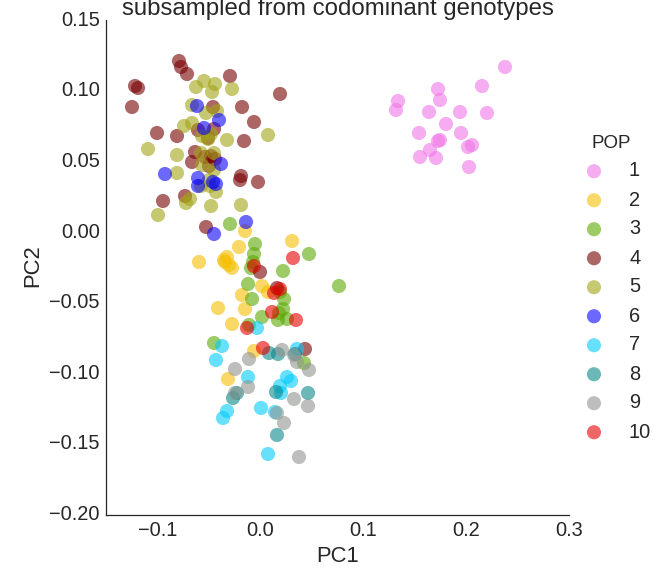
\includegraphics[scale=.3]{figures/PCA_codom_subsample.png}
paralogs have similar neutral patterns of population structure.
measure information loss from dominance coding

discuss population vs individual based results

can we demonstrate contained within paralogs by bootstrapping 
Genome scans - LG regions highlighted.

\subsection*{Effective population size}

\subsection*{Ascertainment Bias}
Demonstrate ascertainment effect when using only loci on linkage map - effect on allele frequencies.

\subsection*{Linkage map}
Identification of paralogs

congruence of identified homeologs across families (supplemental table)

Consensus linkage map

Table (Figure?)
placement of centromeres

table (supplemental)
paralogs
note the distribution of paralogs matches the  pattern found in other salmonids
syntenic relationships - per LG
Table (supplemental?)

\section*{Discussion}
To do

Coalescent!

Does this turn into two papers?

 - linkage map and individual-based analyses - including duplicated loci

 - inference of adaptation -associated  life history variation  - Fst across the genome.

\pagebreak
\section*{Supplemental}

\begin{figure}[H]
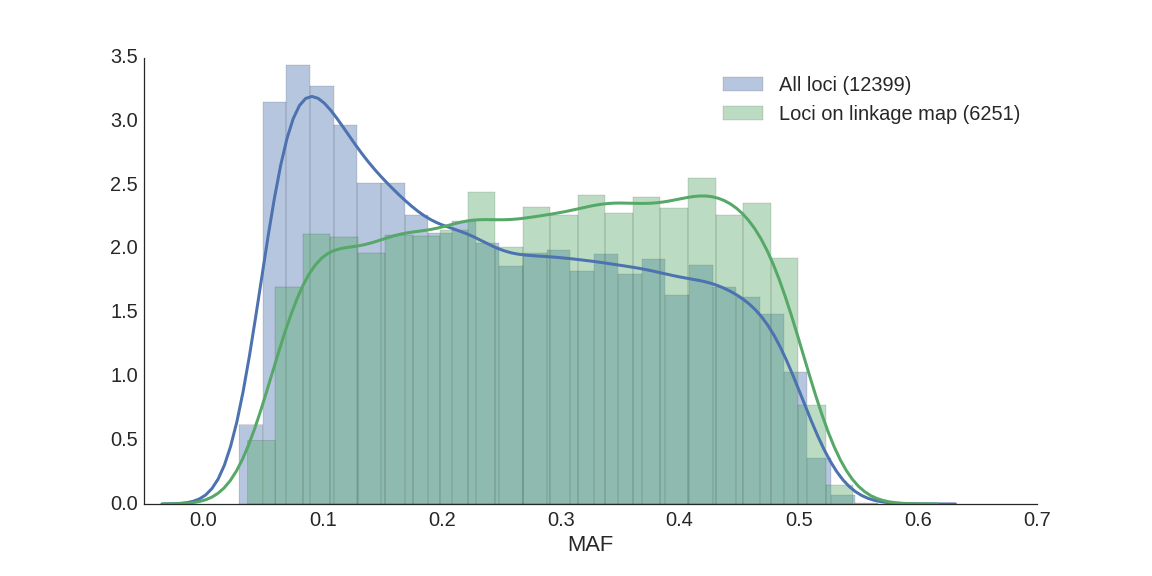
\includegraphics[scale=.3]{figures/supplemental/ascertainment.png}
\caption{Minor allele frequency (MAF) distribution for all genotyped loci (blue) and just the loci placed on the linkage map (green). The rightward shift in the MAF distributino shows the effect of ascertainment bias within the mapped loci.}
\end{figure}

\begin{figure}[H]
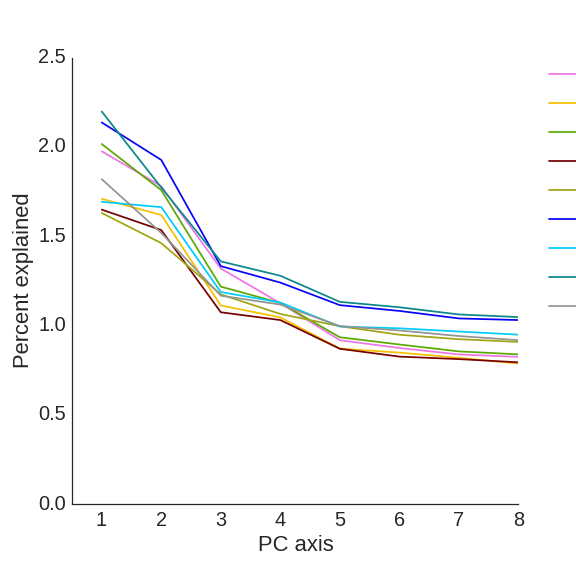
\includegraphics[scale=.4]{figures/supplemental/PCA_eigenvalues.png}
\caption{Percent variance explained (eigenvalue) for the first eight PC axes of each locus set.  Notice the similarity between the two bi-allelic sets and the two haplotypic sets.}
\end{figure}

\begin{figure}[H]
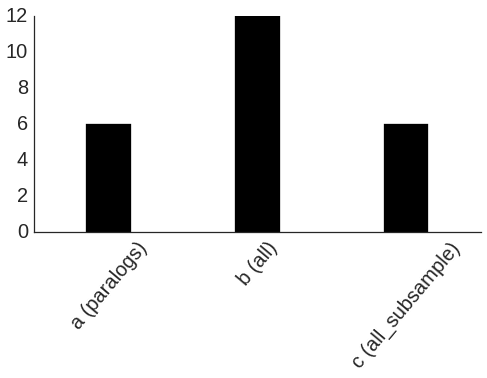
\includegraphics[scale=.4]{figures/supplemental/TW_stats.png}
\caption{Number of significant PC axes as determined by the Tracey-Widom test.}
\end{figure}

\begin{figure}[H]
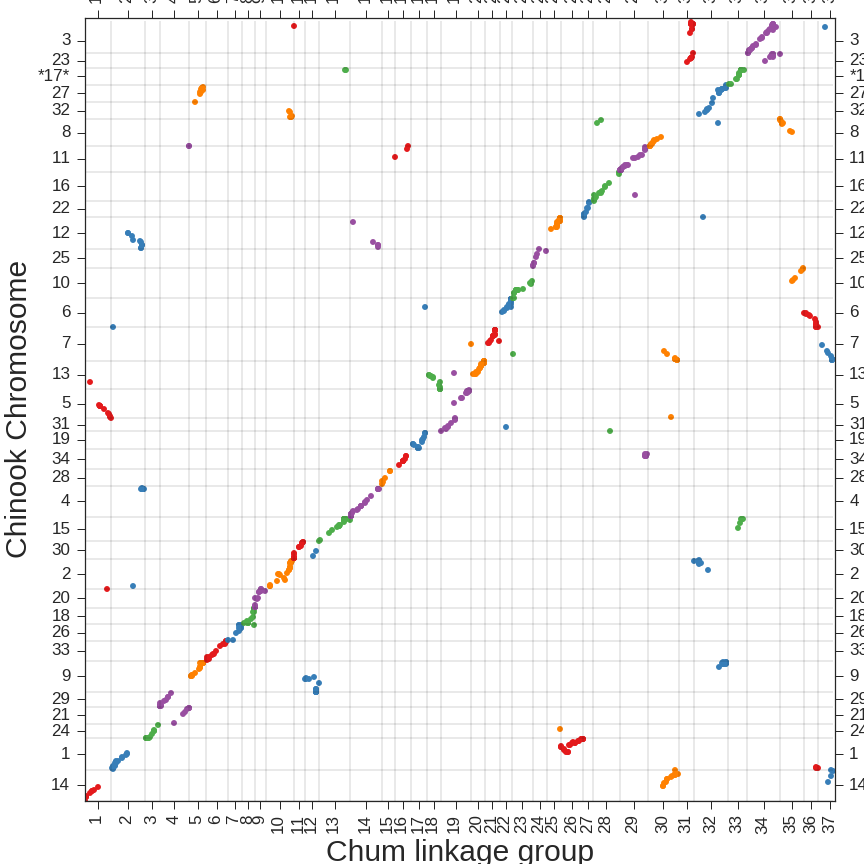
\includegraphics[scale=.25]{figures/supplemental/synteny_chinook.png}
\caption{Oxford grid - Chum and Chinook linkage groups.  Loci are positioned according to the order within each genome.}
\end{figure}

%\begin{figure}
%\begin{center}
%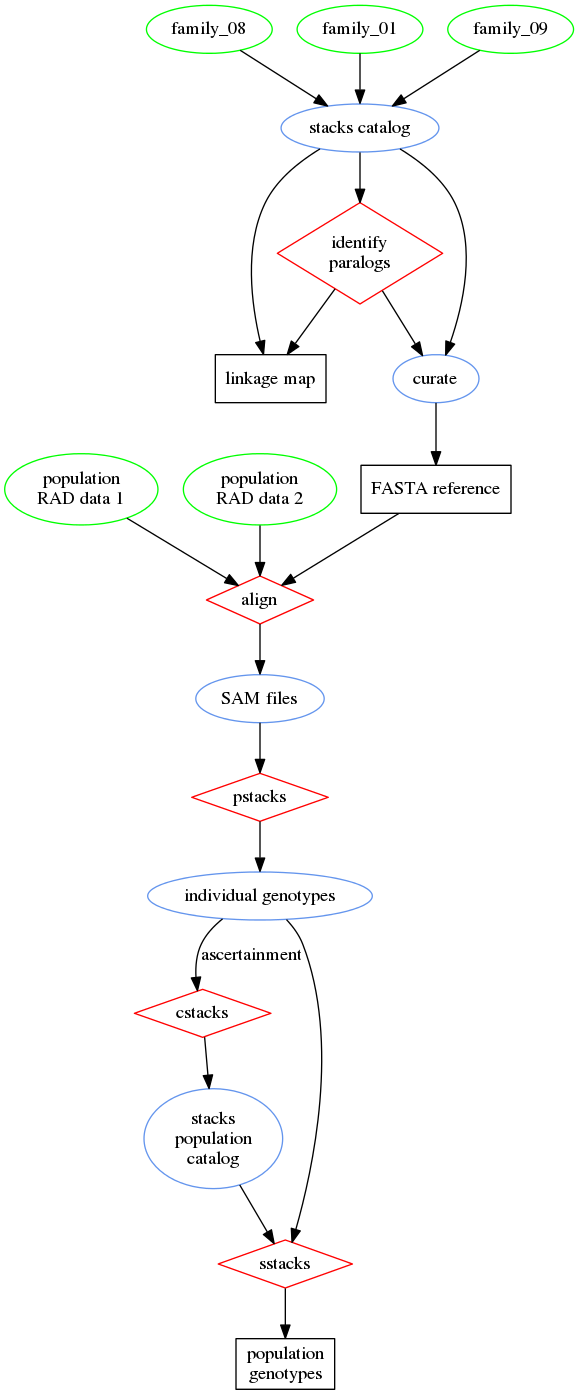
\includegraphics[scale=.3]{figures/supplemental/analysis_flowchart.png}
%\end{center}
%\end{figure}


\end{document}